\chapter{Leader Election}

Il problema della Leader Election consiste nell'avere una configurazione
iniziale del sistema in cui tutte le entità partono dallo stesso stato
(AVAILABLE) e concludere con una configurazione avente tutte le entità nello
stato di FOLLOWER tranne una che sarà nello stato di LEADER.
%Qualche volta è necessario che una determinata entità in un ambiente
%distribuito diventi temporaneamente il controller centrale di tutto il sistema.
%Per far questo, esistono protocolli che fanno in modo che tutte le entità
%partono da uno stesso stato AVAILABLE e al termine del protocollo tutte le
%entità saranno nello stato di FOLLOWER ed uno solo è nello stato di LEADER.\\
LEADER può diventarci qualsiasi entità, poiché non sono presenti restrizioni sul
quale entità deve diventare leader oppure quante entità iniziano la
computazione.
$$P_{INIT}=< \forall x \in \xi, status(x)=AVAILABLE >$$
$$P_{FINAL}=< \exists x \in \xi, status(x)=LEADER \text{ \& } \forall y \neq x
    \text{ , } status(y)=FOLLOWER >$$ La scelta del Leader può essere vista come un
modo per ``forzare'' l'iniziatore unico in tutti i protocolli visti. Esiste,
tuttavia, un risultato di \textbf{impossibilità} sotto R (link bidirezionali,
connettività, e affidabilità totale), ovvero che non esiste un protocollo
deterministico che termina sempre correttamente in tempo finito se le
restrizioni sono solo quelle di R:

\begin{theorem}
    Il problema della Leader Election è deterministicamente non
    risolvibile sotto R.
\end{theorem}

\begin{proof}
    Basta considerare una rete costituita da 2 sole entità identiche, con gli
    stessi numeri di porta e con lo stesso stato (stesso valore iniziale).

    \begin{center}
        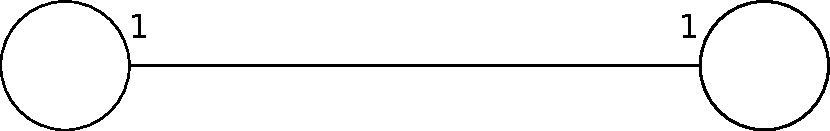
\includegraphics[scale=0.3]{images/n_42}
    \end{center}
    Sia P un protocollo che risolve il problema della Leader Election sotto R,
    questo protocollo deve risolvere il problema sotto qualsiasi circostanza.
    Consideriamo uno scenario in cui le due entità iniziano il protocollo P
    simultaneamente e abbiamo un ritardo di comunicazione unitario. Le due
    entità essendo identiche avranno la stessa esecuzione, se una riceve il
    messaggio anche l'altra lo riceverà e così via, se una diventa Leader anche
    l'altra diventa Leader, ma questo va contro la richiesta, ovvero quella che
    ci deve essere un solo leader, quindi P non è un protocollo che risolve il
    problema.
\end{proof}

La conseguenza di questo teorema è che bisogna rompere la simmetria, ma sotto
R questa simmetria non si riesce a rompere. Il primo approccio sarebbe quello di
aggiungere la restrizione di Inizializzatore Unico, ma in questo caso avremmo
già il leader, e quindi sarebbe inutile applicare il protocollo. Dobbiamo quindi
scartare questa possibilità e modificare le restrizioni in modo tale da
``distinguere'' ogni entità. Per far questo è comune utilizzare una specifica
restrizione, che riguarda l'assegnamento di valori distinti (id) ad ogni entità.
Chiameremo questo nuovo set di restrizioni: Insieme standard per l'elezione:

\begin{definition}
    Si dice \textbf{insieme standard per l'elezione}, l'insieme di
    restrizioni
    \begin{center}
        $IR = R \cup {ID}$
    \end{center}
\end{definition}

\section{Elezione del Leader}
Come possiamo utilizzare questa nuova restrizione per rompere la simmetria ed
eleggere quindi un leader? Analizzando il problema della Leader Election, non
importa quale delle entità diventi Leader, basta che ce ne è una, quindi
utilizzando il fatto che i valori iniziali sono distinti per ogni entità, una
possibile soluzione potrebbe essere quella di scegliere l'entità con il valore
minore:
\begin{itemize}
    \item \texttt{Elect Minimum}
          \begin{enumerate}
              \item Trova il valore più piccolo;
              \item Eleggi come LEADER l'entità con tale valore.
          \end{enumerate}
          Altro approccio:
    \item \texttt{Elect Minimum Initiator}
          \begin{enumerate}
              \item Trova il valore più piccolo tra gli iniziatori;
              \item Elegge come LEADER l'entità con tale valore.
          \end{enumerate}
          Altro approccio ancora potrebbe essere quello di utilizzare i valori
          distinti delle entità per costruire uno spanning tree della rete ed
          eleggere la radice come nodo Leader:
    \item \texttt{Elect Root}
          \begin{enumerate}
              \item Costruisce uno ST radicato;
              \item Elegge come LEADER la radice.
          \end{enumerate}
\end{itemize}

Entrambi i protocolli funzionano \underline{solo} sotto le restrizioni IR,
quindi da qui in avanti prenderemo questo determinato set di restrizioni. Il
problema della leader election dipende dal sistema su cui si stiamo basando.

\section{Election su alberi: utilizzo del protocollo Saturation}
Supponiamo di lavorare su una topologia ad albero, quindi dove $m = n-1$:

\begin{itemize}
    \item Elezione con \texttt{Elect Min}\\
          Abbiamo già visto come trovare in modo ottimale il valore minimo di un
          albero utilizzando la \textbf{Saturazione.} Il protocollo che abbiamo
          studiato si chiama \textbf{MinFind}, supponendo che abbiamo ($K^*$)
          iniziatori il costo della leaderElection tramite questo metodo è:
          \begin{center}
              $M[$\texttt{TreeElectMin}$] = (2n + K^* -2) + (n-2) = 3n + K^* - 4
                  \leq 4n - 4$
          \end{center}
          dove:
          \begin{itemize}
              \item $(2n + K^* -2)$ è il costo della saturazione con $K^*$
                    iniziatori.
              \item $(n-2)$ è il costo del broadcast per comunicare alla rete chi è
                    il Leader.
          \end{itemize}

          La strategia di Elect Minimum Initiator ha lo stesso costo di questo
          approccio.
    \item Elezione con \texttt{Elect Root}\\
          Usiamo i primi due stage della Saturazione per eleggere i due nodi
          saturati, poi questi due si scambiano il loro ID ed il minimo diventa
          LEADER:
          \begin{center}
              $M[$\texttt{TreeElectRoot}$] = (2n + K^* -2) +2 + (n-2) = 3n + k^* - 2
                  \leq 4n - 2$
          \end{center}
\end{itemize}
\begin{itemize}
    \item $(2n + K^* -2)$ Costo normale della Saturazione con $K^*$ iniziatori.
    \item $+2$ Sono i due messaggi che si scambiano i nodi saturi per capire chi
          di loro è il minimo
    \item $n-2$ Notifica in broadcast
\end{itemize}


Dei due metodi è preferibile il secondo se consideriamo la lunghezza in bit dei
messaggi:

In questo approccio solo n messaggi nella Saturazione portano un valore, mentre
tutti gli altri solo segnali. Quindi il numero totale di bit trasmessi sarà:
\begin{center}
    $B[$\texttt{TreeElectMin}$] = n (c + \log_2 id) + c (2n + k^* - 2) = O(n \log
        n + n) = O(n \log n)$\\
    %Dove id denota il valore maggiore inviato in un messaggio e c = O(1) denota
    %il numero di bit richiesti per distinguere tra differenti messaggi. 
    $B[$\texttt{TreeElectRoot}$] = 2(c + \log_2 id) + c(3n + k^* - 2) = O(\log n +
        n) = O(n)$
\end{center}
Nell'elezione tramite la radice, solamente il messaggio di Election porta un ID
di un nodo. Dove:
\begin{itemize}
    \item $c$: bit per rappresentare i segnali (O(1));
    \item $id$: ID più grande da inviare in un messaggio.
\end{itemize}
Quindi in termini di numero di bit, Elect Root è migliore di Elect Minimum.
\section{Election su ring}
Un ring consiste in un ciclo di lunghezza n, dove ogni entità possiede
esattamente due vicini; a livello topologico c'è una totale simmetria delle
entità.\\
L'etichettamento \underline{non} è ordinato (è arbitrario) quindi globalmente le
entità \underline{non} hanno la stessa destra e sinistra ma localmente
distinguono le due direzioni.
\begin{center}
    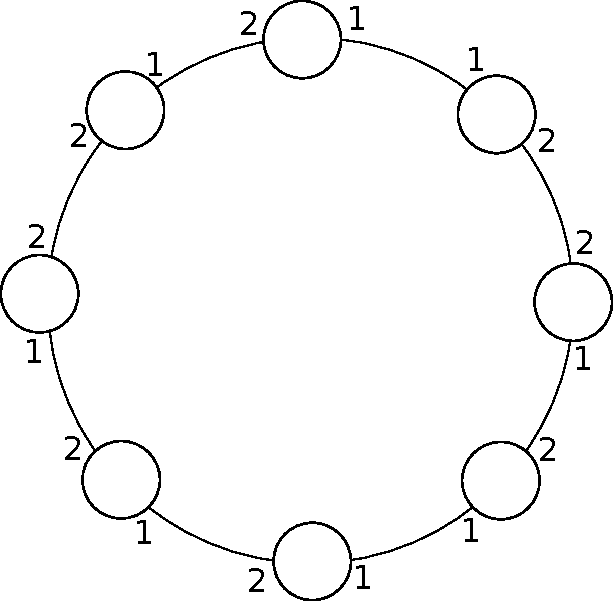
\includegraphics[scale=0.5]{images/n_43}
\end{center}
Consideriamo adesso il problema della Leader Election in un ring chiamato R
sotto le restrizioni IR \{\textit{Bidirectional Links, Connectivity, Total
    Reliability, Initial Distinct Values}\}, ovvero ogni entità ha un valore
iniziale diverso dalle altre.\\ Analizziamo il problema di trovare il minimo e
di eleggere un nodo all'interno di un ring. Chiameremo gli "altri" gli $N(x) - $
sender di un'entità $x$.

\subsection{All The Way: Risoluzione del problema della Leader Election su Ring}
Stati del protocollo:
\begin{itemize}
    \item Asleep, Awake, Follower, Leader
    \item $S_{init}$ = ASLEEP
    \item $S_{term}$ = FOLLOWER, LEADER
\end{itemize}
Quando un'entità inizia, sceglie uno dei due vicini e gli invia un messaggio di
"Election" contenente il suo id; quando un'entità riceve l'id di un altro nodo
propaga il suo e quello che gli è arrivato, tenendo traccia dell'id minimo visto
fino ad ora. Ogni messaggio viaggia fin quando non torna dall'entità che lo ha
spedito.

\paragraph{Terminazione:} Per la terminazione si utilizza un contatore per ogni
entità, per tenere traccia di quanti ID diversi vengono ricevuti, ed un
contatore in ciascun messaggio, in modo che ciascuna entità possa determinare
$n$ quando riceve il suo messaggio dalla parte opposta da quella in cui l'ha
spedito. Quando un'entità ha ricevuto un messaggio da tutte le altre $n$ (ed è a
questo che serve il contatore) sà che ha terminato il protocollo e se ha ID pari
al minimo cambia stato in LEADER. Se un'entità ha l'id maggiore del minimo,
cambia stato in FOLLOWER.

\paragraph{Attenzione:} In questo protocollo non è presente la notifica finale,
un'entità una volta che capisce quante altre entità stanno partecipando al
protocollo (è il valore $n$) saprà se ha ricevuto il messaggio da tutte le
altre. Finché questo non accade non può terminare la sua esecuzione. Quando
invece ha ricevuto un messaggio da tutte le altre può cambiare stato o in LEADER
o in FOLLOWER in base al suo id.

\paragraph{Calcolo del costo:}\ \\
\textbf{Un messaggio originato da ciascuna entità
    viaggerà attraverso tutto il ring esattamente una volta.} Quindi si avranno
esattamente $n^2$ messaggi in totale, ognuno contenente un contatore e un valore
per un totale di $n^2log(id+n)$ bits, per quanto riguarda il tempo invece si
avrà al più 2n. \textbf{Il caso pessimo è quando c'è un unico iniziatore.}\\
\underline{Messaggi:}
\begin{center}
    $M[$\texttt{AllTheWay}$] = n^2$ (è effettivamente =)
\end{center}
\underline{bit:}
\begin{center}
    $B[$\texttt{AllTheWay}$] = n^2*\log_2(id+n)$
\end{center}

Perché ognuno degli $n^2$ messaggi contiene un contatore ed un id. Il contatore
al massimo arriverà ad $n$.

%poiché codifichiamo insieme $id$ (al massimo $n$) e $cont$ (al massimo è $n$).

\underline{Tempo:}
\begin{center}
    $T[$\texttt{AllTheWay}$] \leq (n - 1) + n   = 2n - 1$
\end{center}
\begin{itemize}
    \item (n-1) indica il dover passare tutte le entità meno una per svegliare il
          minimo qualora non fosse già sveglio (caso peggiore).
    \item n invece sono i messaggi inviati dal minimo quando si sveglia.
\end{itemize}

\begin{center}
    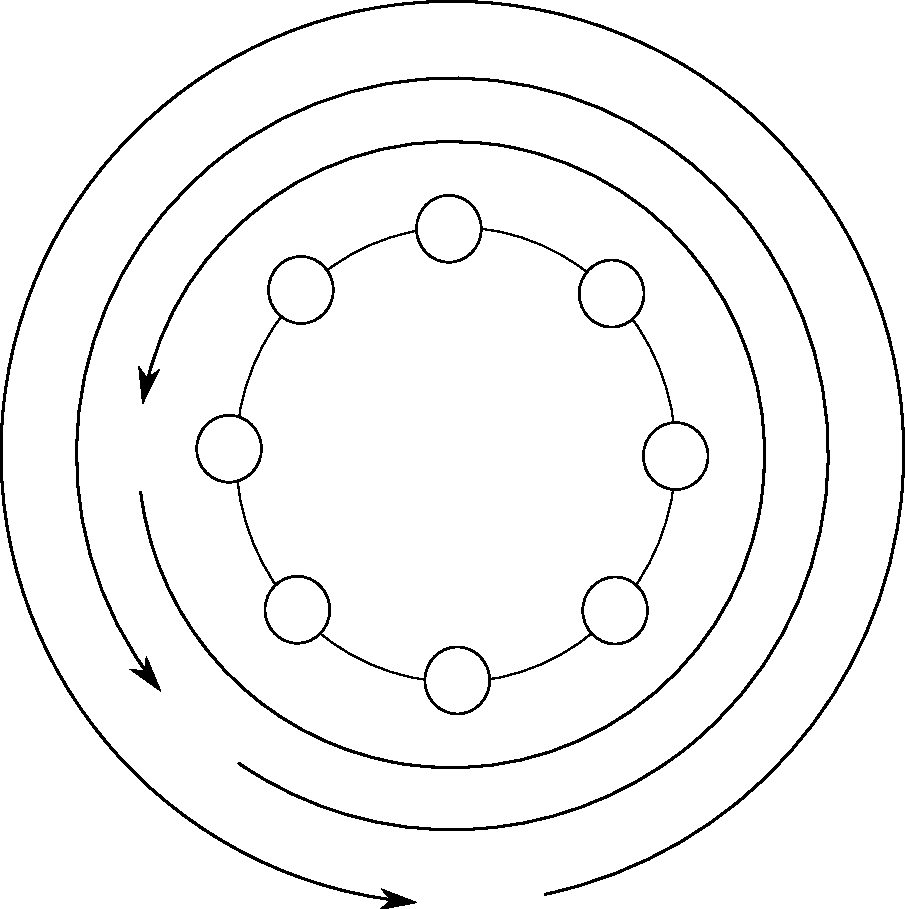
\includegraphics[scale=0.5]{images/n_44}
\end{center}

\paragraph{Risoluzione dell'Elect Minimum Initiator tramite All The Way:} Si deve
trovare il valore minimo tra tutti gli initiator. In questo caso tutte le
\textbf{altre} entità non invieranno nessun messaggio, ma si limiteranno a
propagare solamente il messaggio contenente l'id più piccolo che hanno ricevuto,
non originando quindi nessun messaggio. Bisogna stare attenti però, perché va
modificata la parte del contatore, in quanto non tutte le entità che propagano
possono essere iniziatori. Quindi si ha un problema sulla terminazione. Per come
abbiamo definito il protocollo però, solamente l'effettiva entità che ha $id$
più piccolo riceve un messaggio con il suo stesso $id$ dall'altra parte in cui
ha effettuato la send, quindi questa potrà poi notificare a tutte che il
protocollo può terminare. Questo avviene tramite il messaggio di notifica da
parte del LEADER che farà cambiare stato a tutte le altre entità che partecipano
al protocollo in FOLLOWER.\\
\underline{Messaggi:}
\begin{center}
    $M[$\texttt{AllTheWayMINIT}$] \leq nk^* + n $
\end{center}
\underline{Tempo:}
\begin{center}
    $T[$\texttt{AllTheWayMINIT}$] \leq 3n - 1$
\end{center}
Quindi, qualora ci fosse un unico inizializzatore in questo caso si risparmiano
molti messaggi, ed è il best case che è $O(n)$. Se invece tutte le entità sono
inizializzatori questo protocollo utilizza $n$ messaggi in più dell'altro
metodo.

\subsection{As far as it can}\label{asfar}

Il protocollo inizia con tutte le
entità in stato di AVAILABLE. Queste, quando ricevono un impulso spontaneo
inviano tutte nella stessa direzione il loro messaggio di election che contiene
il loro $id$ e cambiano stato in AWAKE. Un'entità in stato di AVAILABLE riceve il
messaggio di election invia il suo messaggio e controlla se ripropagare anche
quello che gli è arrivato. Se un'entità riceve un ID più grande di quello che ha
visto fino ad adesso non effettua il forwarding di tale messaggio. Tutti gli
iniziatori che iniziano tramite impulso spontaneo scelgono la stessa direzione
nella quale inviare i messaggi, in questo caso \textbf{right}. Se un'entità è in
stato di AVAILABLE = ASLEEP riceve un messaggio di Election allora:

\begin{itemize}
    \item Invia il suo messaggio contenente il suo id all'interno della rete e
          SUCCESSIVAMENTE controlla se ripropagare o no il messaggio che gli è appena
          arrivato.
    \item Per la decisione, controlla se  il valore di tale messaggio è minore del
          minore id che ha visto fino ad adesso. Se così fosse allora effettua il
          forwarding di tale messaggio (generando quindi un nuovo messaggio).
    \item Un'entità in stato di AWAKE, genera messaggi SOLAMENTE se hanno un
          valore più piccolo di tutti quelli visti fino a quel momento.
\end{itemize}

\paragraph{Terminazione:} Siamo sicuri che il protocollo termina poiché solo il
messaggio con ID minimo finisce il giro e solo l'entità con quell'ID saprà di
essere il leader. A questo punto l'unica entità a conoscenza del fatto che il
protocollo può terminare lo comunica agli altri con un singolo messaggio di
notifica ed il protocollo termina essendo eletto il LEADER.

\paragraph{Quando un'entità termina la propria esecuzione?}\ \\
Il messaggio avente id minimo attraverserà sempre tutto il ring, perché nessuna
entità lo fermerà, e quindi sarà l'unico che ritorna al suo mittente. Questo
fatto ci da la possibilità di costruire un meccanismo per far terminare il
protocollo. Se un'entità riceve un messaggio con il suo stesso id, allora sa di
essere il minimo, e quindi il LEADER. Tutte le altre entità avranno visto questo
messaggio, ma non sapranno se potrebbero arrivare altri messaggi contenenti id
più piccoli di quello visto da loro. Quindi per assicurare la terminazione, il
leader invia la notifica in una direzione del link, che attraverserà tutte le
altre entità facendo cambiare stato in FOLLOWER.\\
\underline{Messaggi:}

\begin{center}
    Il LowerBound dei messaggi per la Leader Election è $\Omega(nlogn)$ su sistemi
    Asincroni
\end{center}{}

Ovviamente questo protocollo ha un numero di messaggi minore uguale di quello
precedente, il numero esatto dipende da molti fattori. Considerando il costo del
messaggio di "Election", esso attraverserà il ring fino a quando non trova
un'entità avente id minore oppure completerà il giro. Quindi il costo dipende da
come sono posti gli id all'interno del ring.\\
\textit{Worst Case:} L'id \#1 si sveglia prima di tutti ed invia il messaggio
verso l'entita con id 2. Esso attraverserà sempre tutto il ring, costando n
messaggi. L'id \#2 si fermerà solamente all'entità con id \#1, quindi il costo
nel worst case è $n-1$, ottenibile se l'id \#2 è collocato immediatamente dopo
l'id \#1 nella stessa direzione. In generale quindi l'id \#(i+1) verrà
interrotto da chiunque abbia un id minore e quindi il costo è al più $n-i$
messaggi. Questo succederà se tutte le entità con questi id sono una accanto
all'altra e l'id \#(i+1) è collocato immediatamente dopo la direzione in cui sta
viaggiando il messaggio. Infatti il worst case è \textbf{quando le entità sono
    simultaneamente attivate in ordine "crescente".} Questo implica che il messaggio
con id 1 attraversa n nodi, quello con id 2 ne attraversa n-1 e cosi via
costando $O(N^2)$
\begin{center}
    $M[\texttt{AsFarAsItCan}] = \sum_{i=1}^{n} i + n = \frac{n(n+3)}{2} + n = \in
        O(n^2)$
\end{center}
Dove $n$ è il numero di messaggi per la notifica. $n^2$ lo paghiamo quando siano
particolarmente sfortunati,nel caso medio infatti, con un generico ordinamento,
si ha $O(n \log n)$ (come il QuickSort). Il caso peggiore qui è quando le entità
all'interno del ring sono posizionate in maniera tale da avere il valore in
ordine crescente.

\paragraph{Costo del Tempo: [Siamo ottimi, il Lower Bound è $\Omega(n)$]}
$$T[AsFar,R,id,Ring] \leq n-1 + n + (n-1) = 3n - 1$$ dove:
\begin{itemize}
    \item Dato che non è detto che il minimo si svegli subito, nel caso peggiore
          si sveglierà all'ultimo, quindi diciamo che si "girano" tutti i nodi -1 che è
          proprio il minimo, quando si sveglia il messaggio si bloccherà proprio li.
    \item n indica il giro che farà il messaggio del minimo una volta sveglio.
    \item $n - 1$ indica il giro per la notifica.
\end{itemize}

Possiamo notare che il costo dell'AsFar è uguale a quello dell'All the Way con
l'aggiunta di $n-1$ messaggi per la notifica, che non era presente nell'All the
Way.

\begin{center}
    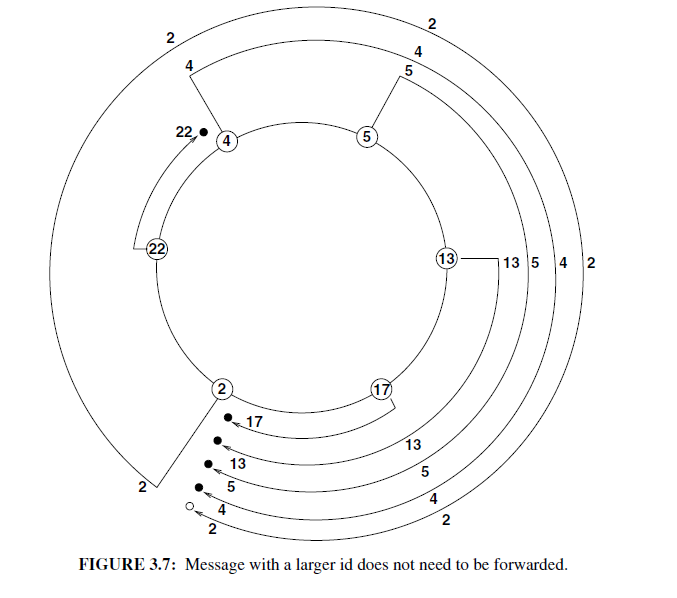
\includegraphics[scale=0.5]{images/asFar.png}
\end{center}

\newpage
\begin{lstlisting} [caption={\textit{Protocollo AsFarAsItCan.}}]
Stati: S = {AVAILABLE, AWAKE, FOLLOWER, LEADER}
$S_{INIT}$ = {AVAILABLE}
$S_{FINAL}$ = {FOLLOWER, LEADER}
Restrictions = R, id, ring

AVAILABLE
    Spontaneously // evento spontaneo
    begin
        send("Election", id(x)) to right
        min := id(x) //il nostro valore
        become AWAKE
    end
    
    Receiving("Election", value) // evento istantaneo
    begin
        if value < id(x) then
            min := value
        else
            min := id(x)
        send("Election", min) to other
        become AWAKE
    end

Procedure NOTIFY
    begin
        send("Notify") to N(x) \ sender
        become LEADER
    end

AWAKE
    Receiving("Election", value)
    begin
        if value < min then
            //alla direzione opposta da dove e' arrivato
            send("Election", value) to other 
            min := value
        else
            if value = id(x) then 
                NOTIFY
            endif
        endif
    end
    
    Receiving("Notify")
    begin
        become FOLLOWER
        send("Notify") to other
    end
\end{lstlisting}

\textbf{Se mandassi il messaggio in entrambe le direzioni?}\\
Un altra idea potrebbe essere di mandare su tutte e due le direzioni e aspettare
che uno solo dei due messaggi rivenga notificato all'entità che l'aveva
mandato.\\
Purtroppo il lowerbound risulta come il precedente, poiché per il nodo con il
minimo potrei avere $2n - 1$, quindi come numero messaggi siamo comunque
nell'ordine di $n^2$, come tempo invece siamo scesi a $n/2 + n$.

\paragraph{Costo del numero di Messaggi:} Il caso peggiore è uguale all'All The Way
asintoticamente, ma si risparmiano alcuni messaggi.
$$\sum_{i=1}^{n} i = \frac{n(n+1)}{2} =  \in O(n^2)$$

\paragraph{Costo del Tempo:} $n/2 + n$\\


\subsection{Controlled Distance}
Sviluppiamo ora un algoritmo che permetterà di risolvere il problema della
Leader Election con un costo di $O(n \log n)$ per il numero di messaggi.
Un'entità manda un messaggio di FORTH contenente la sua candidatura nella due
direzioni, ma entro una distanza limitata. L'entità che invia la candidatura
cercherà quindi di diventare leader di una porzione di rete, se quel messaggio
arriva alla distanza prefissata, l'entità in quella posizione manda un messaggio
di BACK. Se l'entità riceve 2 messaggi di BACK significa che è il minimo in
quella porzione. Se così fosse allora incrementa la distanza iniziando un nuovo
\textbf{stage}, l'obiettivo è quello di diventare leader di tutto il ring.\\
Un'entità diventa DEFEATED se riceve un messaggio avente id più piccolo del suo.
Anche se è sconfitta partecipa comunque al protocollo effettuando il forwarding
dei messaggi delle altre entità ancora in gioco.\\
Se un'entita in stato di CANDIDATE riceve un messaggio con un id più piccolo del
suo diventa automaticamente Defeated indipendentemente dallo stage in cui è. Se
un messaggio torna indietro dall'entità che lo ha inviato ma quell'entità nel
mentre è diventata Defeated allora il messaggio viene semplicemente terminato.\\
Nel caso in cui uno o entrambi i messaggi di BACK non ritornano indietro
l'entità non incrementa il proprio stage, quindi prima o poi riceverà un
messaggio avente id più piccolo del suo diventando DEFEATED.

\paragraph{Correttezza:}\ \\
%Siamo sicuri che questo algoritmo terminerà perché $dis$ è crescente quindi
%prima o poi il detentore del minimo si sveglierà ed il suo messaggio "FORTH"
%gli tornerà indietro e diventerà LEADER. Un'entità che non ha l'id minimo prima
%o poi incontrerà un'entità con un id minore del suo e quindi anche se fosse
%candidata non riceverà due messaggi di BACK e quindi non potrà iniziare un
%nuovo stage. Rimanendo bloccata prima o poi riceverà un messaggio avente id
%minore del suo, e diventerà DEFEATED.
La correttezza dell'algoritmo segue dalla funzione $f: stage \longrightarrow
    distanza $. Il messaggio contenente Id minimo attraverserà sempre un'entità,
indipendentemente dal suo stato (ricordiamo che un'entità in stato di
$candidate$ se riceve un messaggio con id più piccolo diventa automaticamente
$defeated$). Quando la distanza che l'entità avente id minimo può raggiungere
diventa $n$ il messaggio con id minimo viaggia su tutto il ring e quell'entità
riuscirà a diventare LEADER e tutte le altre saranno Defeated.

%Libro: Un'entità x genera un messaggio con il proprio id e questo messaggio
%attraversa il Ring in entrambe le direzioni fin quando o viene terminato o
%quando raggiunge una cerca distanza $f$; se il messaggio non viene terminato si
%ritorna un messaggio di "return" all'entità che lo ha spedito. Quando arriva,
%quell'entità sa di essere quella con l'id minore in quella parte di ring
%delimitata dalla distanza $f$.\\
%%Idee:\\
%%\vspace{-10mm} \begin{itemize} \item Distanza limitata: L'entità imposterà un
%limite sulla distanza di invio del messaggio. \item Messaggi di ritorno: Se
%durante l'attraversamento dell'intervallo limitato il messaggio non viene
%terminato da nessuna entità, in ambe le parti, avente id minore allora si
%invierà il return al nodo originario per "concedere" l'autorizzazione ad
%allungare la distanza possibile. \item Spedisco e verifico su entrambi i versi
%\end{itemize}
\begin{center}
    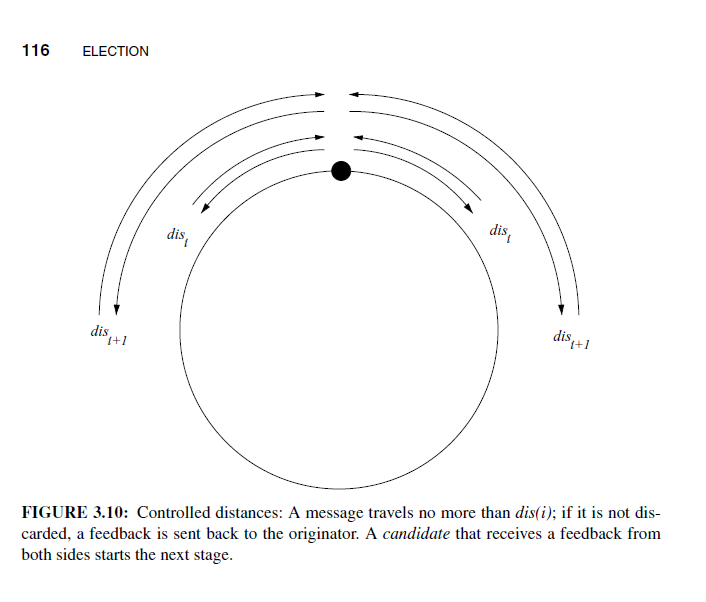
\includegraphics[scale=0.5]{images/controlled.png}
\end{center}
Se si inizia un nuovo Stage, il numero delle entità prese in considerazione sarà
sicuramente maggiore di quelle dello stage precedente, quindi la funzione è
monotona crescente. ($dis(i) > dis(i-1)$).

Riassumendo:
\begin{itemize}
    \item in ogni stato elettorale ci sono alcuni candidati
    \item ogni candidato manda un messaggio in entrambe le direzioni con il
          proprio id
    \item un messaggio viaggia sul ring fin quando non incontra un id più piccolo
          o raggiunge la distanza prefissata
    \item se un messaggio non incontra id più piccoli torna all'entità originante
    \item infine un candidato che riceve entrambi i suoi messaggi in BACKWARD
          inizia un nuovo stage
    \item se un candidato riceve un messaggio (di FORTH) nella direzione opposta a
          quella a cui l'aveva mandato allora diventa LEADER e lo notifica
    \item se un candidato riceve un messaggio con ID più piccolo, diventa DEFEATED
          indipendentemente dallo stadio in cui si trova
    \item un entità sconfitta inoltra i messaggi delle altre entità quando
          necessario, se il messaggio è la notifica lo inoltra e poi termina.
    \item Se un'entità è in stato di ASLEEP e riceve un messaggio di FORTH da
          un'altra entità ma il suo $id$ è minore di quello all'interno del messaggio di
          Forth, allora si cambia stato in CANDIDATE, e si inizia il protocollo.
    \item Se un'entità è in stato di ASLEEP e riceve un messaggio di FORTH da
          un'altra entità ma il suo $id$ è MAGGIORE di quello all'interno del messaggio
          di Forth, allora si cambia stato in PASSIVE, e l'unica cosa che si fa è che si
          inoltrano i messaggi che arrivano.

\end{itemize}

Tipi di messaggio:
\begin{itemize}
    \item Messaggio di candidatura, FORTH
    \item Messaggio di back, BACK
    \item Messaggio di notifica, NOTIFY, che viene spedito in una singola
          direzione.
\end{itemize}

Stati possibili delle entità nel protocollo:

\begin{itemize}
    \item ASLEEP (in p\_{init} tutte le entità sono in questo stato)
    \item CANDIDATE
    \item DEFEATED
    \item FOLLOWER
    \item LEADER
\end{itemize}

Un'entità inizia la propria esecuzione nello stato di ASLEEP. Cambia stato in
CANDIDATE mediante impulso spontaneo e diventa DEFEATED se riceve un ID più
piccolo del suo.\\
Il costo dell'algoritmo dipende totalmente dalla scelta della funzione $f$
utilizzata per determinare la massima distanza in cui viene inviato un messaggio
"Forth" in un determinato Stage.

\subsection{Costo dei messaggi}
\textbf{con $i>1$}\\
%Per avere una stima dei messaggi invece useremo il parametro $n_i$ che indica
%le entità sopravvissute allo stadio $i-1$, cioè le entità che erano candidate e
%sono arrivate allo stadio i-esimo. Vediamo perché questo valore è: $n_i \leq
%\big\lfloor \frac{n}{dis(i-1)+1} \big\rfloor$\\
\textbf{Calcoliamo il massimo numero di entità candidate ad arrivare allo stage $i-esimo$ $n_i$:}
Queste entità sono tutte quelle che hanno superato lo stage $i-1$. Per essere
sopravvissute, l'id dell'entità $x$ deve essere minore di tutti i suoi vicini a
distanza $dis(i)$ in entrambe le parti del ring. Quindi in ogni gruppo di
$dis(i) + 1$ entità consecutive, al più una sopravvivrà lo stage $i-1$ ed
inizierà lo $stage(i)$. Fondamentale che tra due entità in stato di Candidate ci
sono esattamente $dis(i)$ entità comuni. [VEDERE DISEGNO SUL QUADERNO] \\
Ora, quanti insiemi posso avere in un ring? n proprio come il numero delle
entità quindi disequazione:

$$(dis(i-1)+1) * n_i \leq n$$
$$n_i \leq \frac{n}{dis(i-1) + 1}$$

\paragraph{Calcolo dei messaggi allo stage(i):}\ \\
Un'entità che inizia lo $stage(i)$ invierà il messaggio di "FORTH" in entrambe
le direzioni, ogni messaggio viaggerà al più $dis(i)$ di distanza, per un totale
di $2n_i(dis(i))$ numero di messaggi. Esaminiamo ora il messaggi di "BACK": Ogni
entità che sopravviverà a questo stage riceverà tale messaggio in entrambe le
direzioni, le entità che sopravvivranno allo stage(i) sono $n_{i+1}$, quindi
aggiungeranno al totale dei messaggi inviati un $2n_{i+1}dis(i)$ messaggi. Ogni
entità che inizia ma \textbf{non} sopravvive allo $stage(i)$ riceverà o un NO o
un singolo messaggio di "BACK", causando un costo di \textbf{al più} $dis(i)$
messaggi. Il numero di queste entità è $n_i - n_{i+1}$ quindi il numero di
messaggi in questo caso sarà  $(n_i - n_{i+1})dis(i)$. In totale le trasmissioni
di messaggi di "BACK" saranno al più $2n_{i+1}dis(i) + (n_i - n_{i+1})dis(i)$.

\paragraph{Riassumendo:} il numero totale di messaggi inviati allo $stage(i) > 1$
è:
\begin{center}
    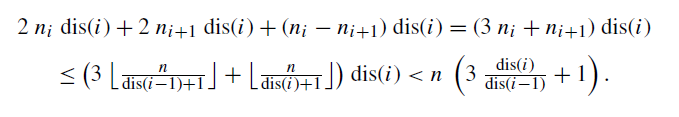
\includegraphics[scale=0.6]{aa/bb.png}
\end{center}
Posso mettere il $<$ perché tolgo il $+1$ sotto, questo mi permette di
semplificare ed infatti viene sempre solamente $+1$.


\subsection{Numero di messaggi inviati al primo Stage (quindi i = 1)}
Il primo stage è differente, poiché ogni entità può essere CANDIDATE; le $n_2$
entità che sono sopravvissute a questo stage avranno causato che i messaggi
contenenti il loro id avranno viaggiato a distanza $dis(1)$ sia per i messaggi
di FORTH che per i messaggi di BACK, causando $4n_2dis(1)$ messaggi. Le $n-n_2$
entità che non sopravvivranno a  questo stage causeranno un costo di al più 3
messaggi ognuno, poiché avremo 2 messaggi di FORTH ed uno solo di BACK nel
peggiore dei casi, quindi avremo $3(n - n_2)dis(1)$ messaggi. Quindi il primo
stage costa:
\begin{center}
    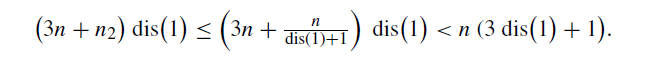
\includegraphics[scale=0.6]{aa/cc.png}
\end{center}
Perché in questo caso $n_2 = n_i$ e quindi il valore può essere sostituito
tenendo conto del $dis(1)$.

\paragraph{Calcolo finale:}
Per trovare il numero di messaggi è necessario essere a conoscenza del numero
totale $k$ di stages. Sappiamo che il leader sarà eletto appena il messaggio con
id più piccolo effettua un giro intero del ring, quindi quando $dis(i) \geq n$.
In altre parole, $k$ è il più piccolo intero tale che $dis(k) \geq n$. Tale
intero è chiamato pseudo-inverso di n ed è denotato da $dis^{-1}(n)$. Quindi il
numero totale di messaggi utilizzati dal protocollo \textbf{Control\_Distance} è
al più:
\begin{center}
    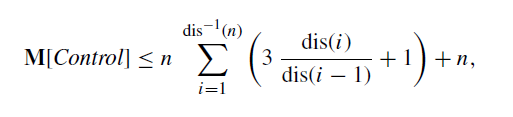
\includegraphics[scale=0.6]{aa/dd.png}
\end{center}
Dove:
\begin{itemize}
    \item $dis(0)$ = 1.
    \item Il $+ n$ finale è il messaggio per la notifica.
\end{itemize}

Per finalizzare il costo bisogna scegliere la funzione $dis$:\\

\paragraph{Funzione Esponenziale: $dis(i) = 2^{i-1}$} e $dis^{-1}(n) =log(n) + 1$
$$\sum_{i=1}^{log(n) + 1 }n(3\frac{2^{i-1}}{2^{i-2}} + 1) = \sum_{i=1}^{log(n) +
        1 }n(3 * 2^{i-1-i+2}+1) =  7nlogn$$ Con la scelta opportuna di $dis$ quindi
siamo riusciti a migliorare il worst case portandolo a $O(nlogn)$.\\

\paragraph{Parole del prof:} Se ci limitiamo a funzioni che fanno un risultato
costante al rapporto $\frac{dis(i)}{dis(i-1)}$, il bound migliore è dato per
$f(i) = 3^i$ e viene $6.309 n log n + n$.

\subsection{Tempo}
Il tempo richiesto dallo $stage(i)$ è il tempo necessario al messaggio
contenente l'id più piccolo per arrivare alla distanza prefissata e tornare
indietro dal suo mittente. Quindi esattamente $2dis(i)$ unità di tempo
necessarie. Un addizionale $n$ va aggiungo sia per la notifica finale, sia per
il wake-up iniziale dell'entità avente il minimo id. Questo quindi comporta che
il tempo totale del protocollo è:
\begin{center}
    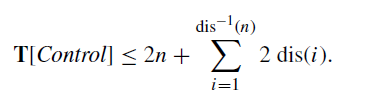
\includegraphics[scale=0.6]{aa/ee.png}
\end{center}
Anche qui dipende dalla scelta della funzione $dis$.

\paragraph{Funzione Esponenziale: $f(i) = 2^{i-1}$}\ \\
Il tempo con questa funzione sarebbe O(n).

% \begin{comment}
% \textbf{Poniamo} dis(1) = Infinito
% $$T[Control\_dis,Ring,R,id] \leq n + \frac{n}{2} + \frac{n}{2}$$ dove:
% \begin{itemize}
%     \item n è per il primo giro (trovare il minimo)
%     \item $\frac{n}{2}$ per trovare il più piccolo nel caso non fosse sveglio
%     \item $\frac{n}{2}$ per la notifica
% \end{itemize}
% \textbf{Poniamo $dis(1) = n/2$.}\\
% $T[$\texttt{Control}$] = \frac{n}{2} + 2n + n$
% \begin{itemize}
%     \item $\frac{n}{2}$ per il wake-up
%     \item $2n$ perché i 2 messaggi FORTH del minimo devono fare tutto il giro
%     \item $n$ per la notifica
% \end{itemize}

% \textbf{Poniamo $dis(1)=n$} allora $T[$\texttt{Control}$] = \frac{n}{2} + n +
%     n$.\\In questo caso si ha il problema che all'inizio del protocollo non si
% conosce il numero delle entità, si può usare un trucchetto che è quello di porre
% $dis(1)$ a infinito.
% \end{comment}

\begin{footnotesize}
    \textbf{Nota: }
    a scopo informativo, esiste un protocollo chiamato \emph{Stages} con un bound
    di $2n log n$, in pratica questo protocollo funziona che ad ogni passo dimezza
    sempre il numero di candidati
\end{footnotesize}

\section{Election su Griglia}
Trattiamo adesso il problema dell'Election su Griglia. Una griglia di dimensioni
$n = a \times b$ ha $a \cdot b$ nodi in cui il generico nodo ha 4 vicini, tranne
quelli ai bordi che ne hanno 3 e quelli negli angoli che ne hanno 2.\\
In una griglia rettangolare si avranno sempre:
\begin{itemize}
    \item 4 angoli: entità con grado 2
    \item $2(a+b-4)$ entità di bordo con grado 3. Dove a sono le colonne mentre b
          sono le righe. il 4 non sono i 4 angoli della griglia, ma sono i 2 angoli
          della prima colonna e i 2 angoli della prima riga, nella figura sottostante
          $x_{1,1}$ viene presa in considerazione quindi due volte.
    \item (a-2)(b-2) entità interne aventi grado 4
\end{itemize}
\begin{center}
    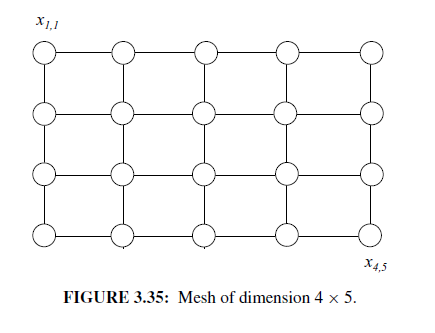
\includegraphics[scale=0.7]{images/griglia.png}
\end{center}

La simmetria di una griglia può essere utilizzata a nostro vantaggio per il
problema della Leader Election. Poiché non importa quale entità diventi leader,
possiamo eleggere uno dei quattro angoli. In questo caso, il problema dello
scegliere il leader su n entità si riduce a trovare il leader tra 4 entità.
L'idea quindi è quella di restringerci alla candidatura solo per gli angoli e
far passare messaggi solo sul bordo così in pratica è come avere un ring. Ci
sono però alcune accortezze da considerare:
\begin{enumerate}
    \item Un initiator non è detto che stia sul bordo.
    \item Se così fosse la prima fase sarà il wake-up così da svegliare tutti i
          nodi compresi gli angoli, che poi faranno le loro candidature tramite l'All
          the Way o l'As\_far o protocollo Stage.
\end{enumerate}
\section{Costruzione del protocollo per Leader Election su Griglia}
Date queste accortezze il protocollo consisterà in:
\begin{itemize}
    \item wake-up che parte dagli iniziatori.
    \item fase di election sul "ring" esterno iniziata dai nodi angolo.
    \item Broadcast della notifica iniziata dal Leader che ha vinto.
\end{itemize}
Nella fase di election gli angoli spediscono in entrambe le direzioni, se chi
riceve è un'entità di grado 2 o 3 allora continua il protocollo, se invece ho
grado 4 (sono interno) o ignoro il messaggio o gli rispondo che sono un nodo
interno e che quindi non mi verranno più inviati messaggi.\\
\subsection{Sviluppo del protocollo}
\begin{enumerate}
    \item Wake-up: Ogni $k^*$ iniziatore invierà un messaggio di Wake-up a tutti i
          suoi vicini, un nodo generico invece che riceverà un messaggio di sveglia da
          uno dei suoi vicini lo ripagherà a tutti tranne la porta dove lo ha ricevuto,
          dato che siamo su una griglia i messaggi inviati da ogni nodo non potranno
          essere più di 3. Per un totale di $3n +k^*$ messaggi inviati.
    \item Elezione su RING e messaggi errati: Bisogna scegliere sia quale
          protocollo utilizzare, sia come gestire i messaggi errati all'interno. Per la
          gestione, si fa in modo che un'entità invii il messaggio su entrambi le porte,
          quindi una sicuramente sarà quella del ring, mentre l'altra si gestisce
          l'errore. Questo farà in modo che l'entità interna che risponde, utilizzi 1
          singolo messaggio, ma così facendo si fa in modo che l'entità nel ring non
          invii più messaggi errati a quella interna.
    \item Broadcast di Notifica: Si può utilizzare il Flooding, che se iniziato da
          uno dei 4 nodi costa $3n$.
\end{enumerate}
Da notare che l'azione più dispendiosa è il wake up iniziale.

\subsection{Calcolo del corso dei Messaggi}
Il numero di Collegamenti all'interno di una griglia è:
$$m=a(b-1)+b(a-1)$$ $M[grid\_leader,R,id,grid] \leq $ wake\_up + elezione +
messaggi sbagliati verso l'interno + notifica in broadcast\\
Mettiamoci nel caso peggiore, ovvero che a svegliarsi sia un nodo interno e che
vengano anche spediti messaggi ai nodi interni dal ring esterno, così da appunto
mandare messaggi inutili.
\begin{itemize}
    \item Costo del Wake Up: Abbiamo $2(m)$ ma in questo caso $m =
              4+3(a+b-4)+2(a-2)(b-2)$.
          \begin{itemize}
              \item $4$ indica gli angoli
              \item 3(a+b-4) indica i nodi di bordo
              \item 2(a-2)(b-2) indica i nodi interni
          \end{itemize}
    \item costo dell'elezione: Utilizziamo il protocollo stage, dato che
          l'elezione è come se avvenisse su un Ring. La proprietà dello stage è che il
          numero di candidati vengono dimezzati quindi avremmo $2n'$ come costo. Siano
          $n'$ i nodi posti solamente sul ring; essi sono un numero pari a $2(a+b-2)$.
          Considerando anche in questo caso gli errori che vengono commessi, un costo
          addizionale di $2(a+b-4)$ messaggi saranno inviati dal bordo verso i nodi
          interni, che dovranno rispondere un "Non mandarmi più messaggi perché hai
          sbagliato" e quindi la risposta costa altri $2(a+b-4)$ messaggi. In
          conclusione il numero di messaggi che verranno inviati in questa fase sono:
          $$4(a+b-2)+2(a+b-4) = 6(a+b)-16$$
    \item Broadcast della notifica: Dato che sappiamo che l'UI è esattamente un
          angolo, esso invierà sempre 2 messaggi. un nodo generico manda la notifica in
          broadcast sempre su due link poiché i nodi interni aspettano esattamente due
          notifiche, ogni nodo quindi manda esattamente due messaggi. Così facendo il
          costo del broadcast è esattamente $2n$.\\\\La notifica costa: $2m - n +1 = 2
              (2ab -b-a) -ab +1 = 3ab-2a-2b+1 \approx 3n$\\
          Per la notifica si può fare che i nodi sul bordo inviano solo 2
          messaggi, quelli interni aspettano l'arrivo di 2 messaggi e poi ne
          inviano altri 2, sugli archi da cui non gli sono arrivati. Quindi
          possiamo scendere a $2n$ messaggi per la notifica.
\end{itemize}
In conclusione, la fase più dispendiosa è il Wake Up iniziale che costa $4n$\\\\
Se a svegliarsi non sono i nodi sul bordo, essi andranno svegliati tramite un
wake-up.\\
$m = a(b-1) + b(a-1)$, quindi per il wake-up si spenderebbero all'incirca $2n$
messaggi.

Per far viaggiare il protocollo di Leader Election solo sul bordo si potrebbe
fare che i nodi esterni, quando ricevono un messaggio di candidatura, inviano 2
messaggi nei link che gli sono rimasti, uno rimarrà quindi nel bordo e proseguirà nel
protocollo, l'altro direzionato all'interno della griglia verrà quindi ricevuto
da un entità che sa di essere un nodo interno, ignorerà quindi il messaggio.

Se un entità riceve un messaggio di BACK sa che esso proviene da un entità di
bordo e quindi potrà conoscere la sua effettiva situazione degli archi.

Se applichiamo \emph{Stages} avremo $\mathcal{O}(2n' \log n')$ con $n' = 2a + 2b
    - 4$ e con 2 stadi elettorali abbiamo eletto il leader.

\section{Election su Grafi Completi}
Affrontiamo adesso il problema della Leader Election con una topologia a grafo
completo. Se usassimo un algoritmo standard saremmo nell'ordine di $n^2$.
Risolvere la leader election ha come conseguenza diretta quella di risolvere il
wake-up, il lower-bound per questo nei grafi completi avevamo visto essere
$\Omega(\frac{1}{2}n \log n)$ tramite la tecnica dell'avversario.

\paragraph{Insieme delle restrizioni:} Insieme standard per l'elezione. $(R+ID)$\\
Per costruire un protocollo più efficiente per l'ELECTION in un grafo Completo
utilizzeremo una tecnica chiamata \textbf{Territory Acquisition.}\\
L'insieme degli stati in questa tecnica è il seguente:

\paragraph{Stati:} \{LEADER, FOLLOWER, ASLEEP, CANDIDATE, PASSIVE, CAPTURED\}

\paragraph{Descrizione a parole:}
In questa tecnica abbiamo un certo numero di candidati dove ognuno di essi prova
a "catturare" i suoi vicini \textbf{uno alla volta} tramite l'invio di messaggi
"CAPTURE" contenenti l'id del mittente ed il numero di nodi catturati fino ad
ora (lo \textit{Stage)}. Se il tentativo va a buon fine, l'entità che ha
ricevuto il messaggio diventa "Captured" e il candidato entra in un nuovo Stage
continuando la sua esecuzione. Altrimenti il candidato diventa "Passivo".
Trattandosi di un protocollo sequenziale, ovvero che una singola entità alla
volta può essere conquistata da un'altra in stato di CANDIDATE, e trovandoci su
grafo completo, appena un'entità possiede uno stage di valore $\frac{n}{2} +1 $
allora cambia stato in LEADER ed invia un messaggio di "notifica" a tutti i suoi
vicini (ovvero a tutte le entità del sistema dato che siamo su grafo completo).
Fondamentale il fatto che se due entità hanno lo stesso stage, allora vince chi
ha l'id più PICCOLO.\\
Riassumendo: Un'entità in un qualsiasi momento può essere "Candidate",
"Captured" o "Passiva". Un'entità Captured ha in memoria \textbf{l'id, lo stage}
ed il collegamento al suo "possessore", ovvero l'entità che l'ha catturata. Le
entità che sono CANDIDATE lo diventano tramite impulso spontaneo in stato di
ASLEEP. Di seguito le \textbf{regole formali:}
\begin{enumerate}
    \item Un entità candidata x manda un messaggio di CAPTURE ad un suo vicino y
          (che non fa già parte del territorio di x)
    \item Se y è passivo o Asleep l'attacco ha successo. x incrementa il suo stage
          ed y diventa Captured.
    \item Se y è "CANDIDATE", il risultato dell'attacco dipende dallo stage e
          dall'id delle due entità:
          \begin{itemize}
              \item Se $stage(x) > stage(y)$, l'attacco ha successo. x incrementa il
                    suo stage ed y diventa Captured.
              \item Se $stage(x) = stage(y)$, l'attacco ha successo se $id(x) <
                        id(y)$ altrimenti $x$ diventa passivo.
              \item Se $stage(x) < stage(y)$, x diventa passivo.
          \end{itemize}
    \item Se y è "CAPTURED" allora x deve sconfiggere il padrone di y, che
          chiameremo z, prima di poter catturare y. Se così fosse, y manda a z un
          messaggio di WARNING con stage(x) e l'id(x) e:
          \begin{itemize}
              \item Se z è candidato in uno stage più alto o nello stesso stage di x
                    ma $id(z) < id(x)$ allora l'attacco a y da parte di x non ha successo.
                    z quindi lo notifica a y che lo notifica a x.
              \item In tutti gli altri casi (ovvero se z è già stato a sua volta
                    catturato, se z è passivo, se z è un "Candidate" in uno stage più
                    piccolo o ha lo stesso stage di x ma con id più grande di x) l'attacco
                    ha successo; z lo notifica a y che lo notifica a x e se z era
                    candidato diventa passivo (dato che z poteva già essere "Passivo").
          \end{itemize}
    \item Se l'attacco ha successo, y è catturata da x, x incrementa il suo
          $stage(x)$ e continua l'esecuzione della sua conquista.
          %\item Quando una delle entità diventa il leader, lo notifica tramite
          %broadcast a tutte le altre.
\end{enumerate}
Al protocollo va aggiunta poi la notifica finale. \\
\subsection{Costo dei Messaggi}
Da notare che ogni tentativo effettuato da un Candidato ad un vicino anch'esso
"Candidato" o "Passivo" costa esattamente due messaggi:
\begin{itemize}
    \item Uno per "Capture".
    \item Uno per la Notifica.
\end{itemize}
Se invece il suo vicino è già stato Catturato, due messaggi addizionali verranno
inviati:
\begin{itemize}
    \item Uno dall'entità già catturata al suo padrone.
    \item Il messaggio di ritorno dal Padrone all'entità.
\end{itemize}
Questo metodo risolve quindi il problema dell'elezione sui grafi completi.

\subsection{Descrizione a parole del protocollo}

\begin{itemize}
    \item \textbf{AVAILABLE:} Se ricevi impulso spontaneo allora fissa lo stage =
          1, il valore = id(x) e crea l'insieme "others" che contiene tutto il tuo
          vicinato. Scegli un nodo dentro questo insieme ed invia il messaggio di
          Capture a quest'ultimo allegando il suo stage ed il tuo id. Successivamente
          diventa CANDIDATE.\\
          Se invece non ti svegli tramite impulso spontaneo ma ricevi un messaggio
          di Capture da Available allora invia immediatamente il messaggio di
          accettazione salvando l'entità che è tua "padrona", il tuo stage che è =
          1 e lo stage del tuo padrone +1 (puoi vedere questo valore perché te lo
          ha inviato all'interno del messaggio). Successivamente cambia stato in
          CAPTURED.
    \item \textbf{CANDIDATE:} Se ricevi un messaggio di tipo "Capture" allora fai
          tutti i controlli sopra. Da notare che se chi attacca vince questa entità
          diventa CAPTURED.\\
          Se invece ricevi un messaggio di "ACCEPT" allora incrementa il suo stage
          e controlla subito se questo valore è $\geq \frac{n}{2} +1$. Se cosi
          fosse invia la notifica a tutti i tuoi vicini (che sono tutte le entità
          dato che siamo su un grafo completo) e diventa Leader. Altrimenti il tuo
          stage non è grande a sufficienza per vincere, prova quindi ad inviare un
          altro messaggio di Capture ad un altro dei tuoi vicini.
    \item \textbf{Candidate:} Se ricevi il messaggio di "reject" cambia stato in
          PASSIVE. \\ Se ricevi il messaggio di "Terminate" cambia stato in
          FOLLOWER. \\ Se ricevi uno "Warning" significa che un'entità sotto il
          tuo controllo è stata attaccata da un altra in stato di CANDIDATE,
          effettua i controlli sopra ed invia "NO" o "YES" in base a questi.
    \item \textbf{Passive:} Se ricevi un messaggio di CAPTURE hai comunque in
          memoria lo stage dell'ultima entità che ti ha conquistato, quindi controlla
          comunque se lo stage e l'id dell'entità che prova a conquistarti ora sono
          validi (fai i controlli precedenti). Se i controlli vanno a buon fine diventa
          nuovamente CAPTURED salvando lo stage del tuo possessore e quale è il tuo
          possessore.
\end{itemize}

\subsection{Calcolo del costo}
È necessario tenere traccia di quanti candidati possono essere presenti allo
$stage(i)$. Rappresentiamo questo valore con $n_i$. Per calcolare questo valore
però è necessario assicurare che un nodo venga catturato da al più 1 candidato
nello stesso stage.\\
\textbf{Vediamo un esempio del problema del protocollo appena enunciato:}\\
Supponiamo quattro entità x, y, z, w; x e y sono nello stesso stage e z è
catturata da w.\\
Se sia x che y mandano un messaggio di candidatura a z, questa allora manderà un
WARNING a w e verrà poi notificata la risposta, supponiamo poi che prima che
arrivi il messaggio di notifica, z processa anche y e manda quindi un altro
WARNING a w, a questo punto abbiamo 2 notifiche da parte di w, queste possono
essere entrambe positive. Ci ritroveremmo quindi che sia x che y hanno
conquistato z, ma secondo z essa è legato solo all'ultima processata, quindi
y.\\
\subsubsection{Risoluzione del problema:}
Possiamo ovviare a questo problema mettendo un buffer nelle entità. Facciamo in
modo che i messaggi di Warning siano inviati uno alla volta e solamente al vero
padre dell'entità che sta venendo conquistata Facciamo in modo un'entità aspetti
dopo un WARNING quale sia la risposta ricevuta, così nello stesso caso di sopra
la nuova domanda (di y) sarebbe stata mandata al vero candidato, cioè x.\\
Apportiamo le seguenti modifiche:
%S\vspace{-5mm}
\begin{enumerate}
    \item Se un nodo catturato y riceve un messaggio di CAPTURE da un candidato x
          che è in uno stadio più piccolo di quello conosciuto da y, allora y notifica
          immediatamente a x che l'attacco non ha avuto successo (x diventa passivo). Di
          conseguenza, un nodo y catturato invierà solo WARNING per un attacco che ha
          stage più alto del suo.
    \item Se un nodo y manda un WARNING al suo padrone z riguardante un attacco di
          x, allora y aspetta la risposta da z prima di mandare eventuali altri WARNING.
\end{enumerate}
La conseguenza di questo secondo punto è che se un attacco da x ha successo (e
quindi il suo stage viene incrementato) y invierà al nuovo padrone x qualsiasi
WARNING successivo generato dall'elaborazione dei messaggi di cattura accodati.
Dopo questa modifica, è garantito che il territorio di due candidati nello
stesso stage non abbia nodi in comune.\\

\colorbox{yellow}{\textbf{Quanti candidati possono essere presenti allo stage
        i?}}\\
Ogni candidato ha un territorio di grandezza i e questi territori sono
disgiunti, quindi non possono esserci più di $$n_i \leq \frac{n}{i}$$ candidati
(Le entità vengono conquistate una alla volta, il protocollo è sequenziale). \\

\colorbox{yellow}{\textbf{Quanti messaggi inviano $n_i$ candidati allo
        $stage(i)$?}}\\
Ognuno darà origine ad un attacco che costerà al massimo 4 messaggi; quindi,
nello stage i, ci saranno al più $$\frac{4n}{i}$$ messaggi. \\

\colorbox{yellow}{\textbf{Determiniamo ora il numero di Stage necessari per la
        terminazione del protocollo.}} \\
Consideriamo il seguente fatto: Se un Candidato ha conquistato un territorio di
grandezza $$\frac{n}{2} +1,$$ nessun altro candidato può diventare Leader.
Quindi, un candidato può diventare leader appena raggiunge quello stage
(successivamente fa il broadcast della notifica di "vittoria" a tutti gli altri
nodi).\\

In conclusione, il numero totale di messaggi, incluso $n-1$ messaggi per la
notifica finale in broadcast è il seguente:

$$ n-1 + \sum_{i=1}^{\#stadi} 4 n_i \leq n-1 + 4 \sum_{i=1}^{n/2} n_i = 4 n
    H_{n/2} + n + 1$$ Dove:
\begin{itemize}
    \item (n-1) è il costo della notifica in broadcast su un grafo completo,
          ovvero l'entità LEADER invia un messaggio a tutti i suoi vicini che sono
          $n-1$.
    \item La sommatoria indica i messaggi inviati dalle entità candidate allo
          stage(i) che sono appunto al più 4 per ognuna di esse.

\end{itemize}

Che da un costo complessivo di:
$$M[CompleteElection, R, id, K_n] \leq 2.76 n log n - 1.76 n + 1$$ Il costo del
libro è il seguente:\\
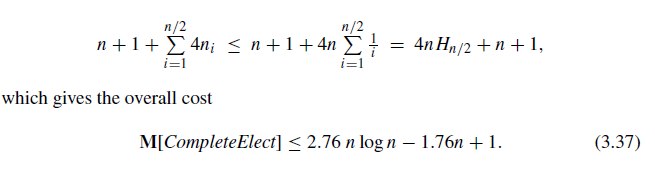
\includegraphics[]{images/fff.png}
Dal libro e dagli appunti presi a lezione, ne risulta che la serie è un'armonica
crescente, che ha come risultato $nlogn$, credo che sia questo il $H_{n/2}$
sulla foto del libro.\\

\textbf{Siamo ottimi per i messaggi?}
SI! perché il lower bound per QUALSIASI protocollo di Leader Election su grafo
completo è $\Omega(n \log n)$ messaggi, dato che ha come sotto problema quello
del Wake-Up, ovvero che tutte le entità, prima di eleggere il Leader devono
necessariamente essere sveglie. Abbiamo visto tramite la tecnica dell'avversario
che il Lower Bound per il Wake-up è $\frac{1}{2}n \log n$.\\


\textbf{Tempo:}\\ $$T[CompleteElection, R, id, K_n] \leq 4 \frac{n}{2} + 1 \leq
    2 n$$
\begin{itemize}
    \item $ 4 \frac{n}{2} $ Perché abbiamo 4 messaggi per stage nel caso peggiore.
    \item + 1 indica la notifica finale che, essendo in un grafo completo, costa
          una singola unità di tempo.
\end{itemize}

\paragraph{Siamo ottimi per il tempo?} NO! perché è possibile sviluppare un
protocollo che ogni entità invia l'id a tutti i suoi vicini (che sono n-1 in un
grafo completo) e poi tutti rispondono con un messaggio contenente il loro ID,
così che ogni entità possa determinare se il suo è l'id minimo oppure no. In
questo caso spediamo $O(1)$ tempo ma il costo dei messaggi va a $O(n^2)$.

\subsection{Miglioramento del protocollo Complete Election: tolgo la sequenzialità e riesco ad abbassare il tempo}
Il protocollo che abbiamo appena visto impone che ad ogni singolo stage
un'entità possa conquistarne esattamente un'altra, quindi abbiamo in gioco il
fattore della sequenzialità. Per effettuare una miglioria sul tempo è necessario
ridurre il numero di stage. Per far questo però è necessario togliere la
sequenzialità, ovvero fare in modo che in ogni stage un'entità deve cercare di
conquistarne più di un'altra.\\

\textbf{Caso Estremo:} Abbiamo un singolo iniziatore che contatta tutti, il
tempo in questo caso sarebbe $O(1)$ ma il numero dei messaggi salirebbe a
$O(n^2)$. Ne risulta quindi che bisogna porre un limite sulle entità
contattabili.\\

\textbf{Creazione dell'algoritmo migliore:} Vediamo adesso come creare
un'algoritmo che ci consenta di avere $O(n \log n)$ messaggi e $O(\log n)$
tempo.\\
Facendo riferimento alle domande poste durante lo sviluppo del precedente
protocollo:\\

\textbf{Quanto è il numero delle entità candidate contemporaneamente allora
    stage i-esimo?}: Esattamente $n_i$. Se allora stage i-esimo si conquistano $2^i$
entità allora $n_i = \frac{n}{2^i}$. Così facendo il numero di messaggi inviati
raddoppia ma il numero delle entità che li mandano dimezza, e quindi siamo
restati sulla stessa complessità. Al più la metà delle entità che si sveglia
passa allo stage successivo.
\begin{center}
    Costo dei Messaggi: $O(n \log n)$\\
    Costo del tempo: $O(\log(n))$
\end{center}
